\chapter{Commande des robots manipulateurs II: dynamique}

Ce chapitre présente des techniques de commande qui s'applique pour les systèmes robotisés où les entrées du système sont des forces ou couples produites par les actionneurs. Dans ce contexte, le système peut être modéliser comme un système d'équations différentielles non-linéaire d'ordre deux et être représentés par l'équation des manipulateurs décrite au chapitre \ref{sec:dynamic}.  Les vidéos suivants présentent une introduction, avec un point de vue graphique dans l'espace des phases, aux méthodes pour se contexte:

\video{Introduction à la commande des robots}{https://youtu.be/eL6i319X_w4}
\video{L'espace des phases}{https://youtu.be/eL6i319X_w4}
\video{Tour d'horizon des méthodes de commande dans l'espace des phases}{https://youtu.be/eL6i319X_w4}

Au lien suivant, une amorce de code pour tester des lois de commande sur un robot manipulateur à 2 DDL:
\colab{Testez votre loi de commande pour un manipulateur}{https://colab.research.google.com/drive/1bnJ9v5kHRFFhnNOZx-_Kcht2l5sTOHxr?usp=sharing}




\newpage
%%%%%%%%%%%%%%%%%%%%%%%%%%%%%%%%%%%%%%%%%%%%%%%
\section{Commande dé-localisée}
%%%%%%%%%%%%%%%%%%%%%%%%%%%%%%%%%%%%%%%%%%%%%%%

Dans certains situations, il est possible de traiter le problème de commande joint par joint avec des méthodes de commande classique comme des lois de commandes de type PID. Cette approche peut bien fonctionner surtout lorsque le système robotique a des actionneurs avec des grands ratios de réduction, ce qui minimise le couplage dynamique entre les divers DDL. Plus les effets inertiels et plus on désire suivre précisément des trajectoires dynamiques, moins ce type d'approche va être performante.

\colab{Simulation d'un manipulateur avec des PIDs }{https://colab.research.google.com/drive/1qaCNY2ohQIbC6dV2ZW4KY6FDM9NhJzH2?usp=sharing}

Détails à venir!


\newpage
%%%%%%%%%%%%%%%%%%%%%%%%%%%%%%%%%%%%%%%%%%%%%%%%%%%%%
\section{Commande avec la méthode du couple calculé}
%%%%%%%%%%%%%%%%%%%%%%%%%%%%%%%%%%%%%%%%%%%%%%%%%%%%%

La méthode du couple calculé consiste à utiliser les équations d'un modèle dynamique d'un système robotique pour déterminer les forces à appliquer pour obtenir une accélération cible. Il est ensuite possible de calculer cette accélération cible de sorte à converger vers la position ou trajectoire désirée.

\video{Méthode du couple calculé}{https://youtu.be/QuEhwAUxx5Y}


\colab{Robot avec une loi de commande du couple calculé}{https://colab.research.google.com/drive/19SLbtnJHDen3-EUIyP1BSFVhGs4WSc5J?usp=sharing}


\subsection{Commande de l'accélération des joints}

Premièrement, si un système est pleinement actionné, il est possible d'imposé d'une accélération arbitraire dans l'espace des joints à un instant donné. Pour un système décrit par l'équation des manipulateurs:
%%%%%%%%%%%%%%%%%%%%%%%
\begin{align}
H(\col{q}) \col{\ddot{q}} + C(\col{q},\col{\dot{q}}) \col{\dot{q}} + d(\col{q}, \col{\dot{q}}) + \col{g}(\col{q}) = B(\col{q}) \col{u} 
\end{align}
%%%%%%%%%%%%%%%%%%%%%%%
si on définie une loi de commande avec une accélération référence $\col{\ddot{q}}_r$:
%%%%%%%%%%%%%%%%%%%%%%%
\begin{align}
\col{u} = B(\col{q})^{-1} \left[  H(\col{q}) \col{\ddot{q}}_r + C(\col{q},\col{\dot{q}}) \col{\dot{q}} + d(\col{q}, \col{\dot{q}}) + \col{g}(\col{q}) \right]
\end{align}
%%%%%%%%%%%%%%%%%%%%%%%
qui assume ici que la matrice $B$ est inversible, donc que le système est pleinement actionné. Alors si on substitut la loi de commande dans l'équation de la dynamique on obtient:
%%%%%%%%%%%%%%%%%%%%%%%
\begin{align}
H(\col{q}) \col{\ddot{q}} + C(\col{q},\col{\dot{q}}) \col{\dot{q}} + d(\col{q}, \col{\dot{q}}) + \col{g}(\col{q}) &= B(\col{q}) B(\col{q})^{-1} \left[  H(\col{q}) \col{\ddot{q}}_r + C(\col{q},\col{\dot{q}}) \col{\dot{q}} + d(\col{q}, \col{\dot{q}}) + \col{g}(\col{q}) \right]  \\
H(\col{q}) \col{\ddot{q}} &= H(\col{q}) \col{\ddot{q}}_r \\
\col{\ddot{q}} &= \col{\ddot{q}}_r
\end{align}
%%%%%%%%%%%%%%%%%%%%%%%
on obtient comme résultat que l'accélération du système peut être directement commandée. Comme illustré à la figure \ref{fig:computedtorque}, avec cette loi de commande, la relation entre la référence $\col{\ddot{q}}_r$ et la variable à contrôler $\col{q}$ est réduite à une relation linéaire, ici un double intégrateur. On réfère aussi parfois à cette méthode comme une boucle linéarisante.

%%%%%%%%%%%%%%%%%%%%%%%%%
\begin{figure}[htp]
	\centering
		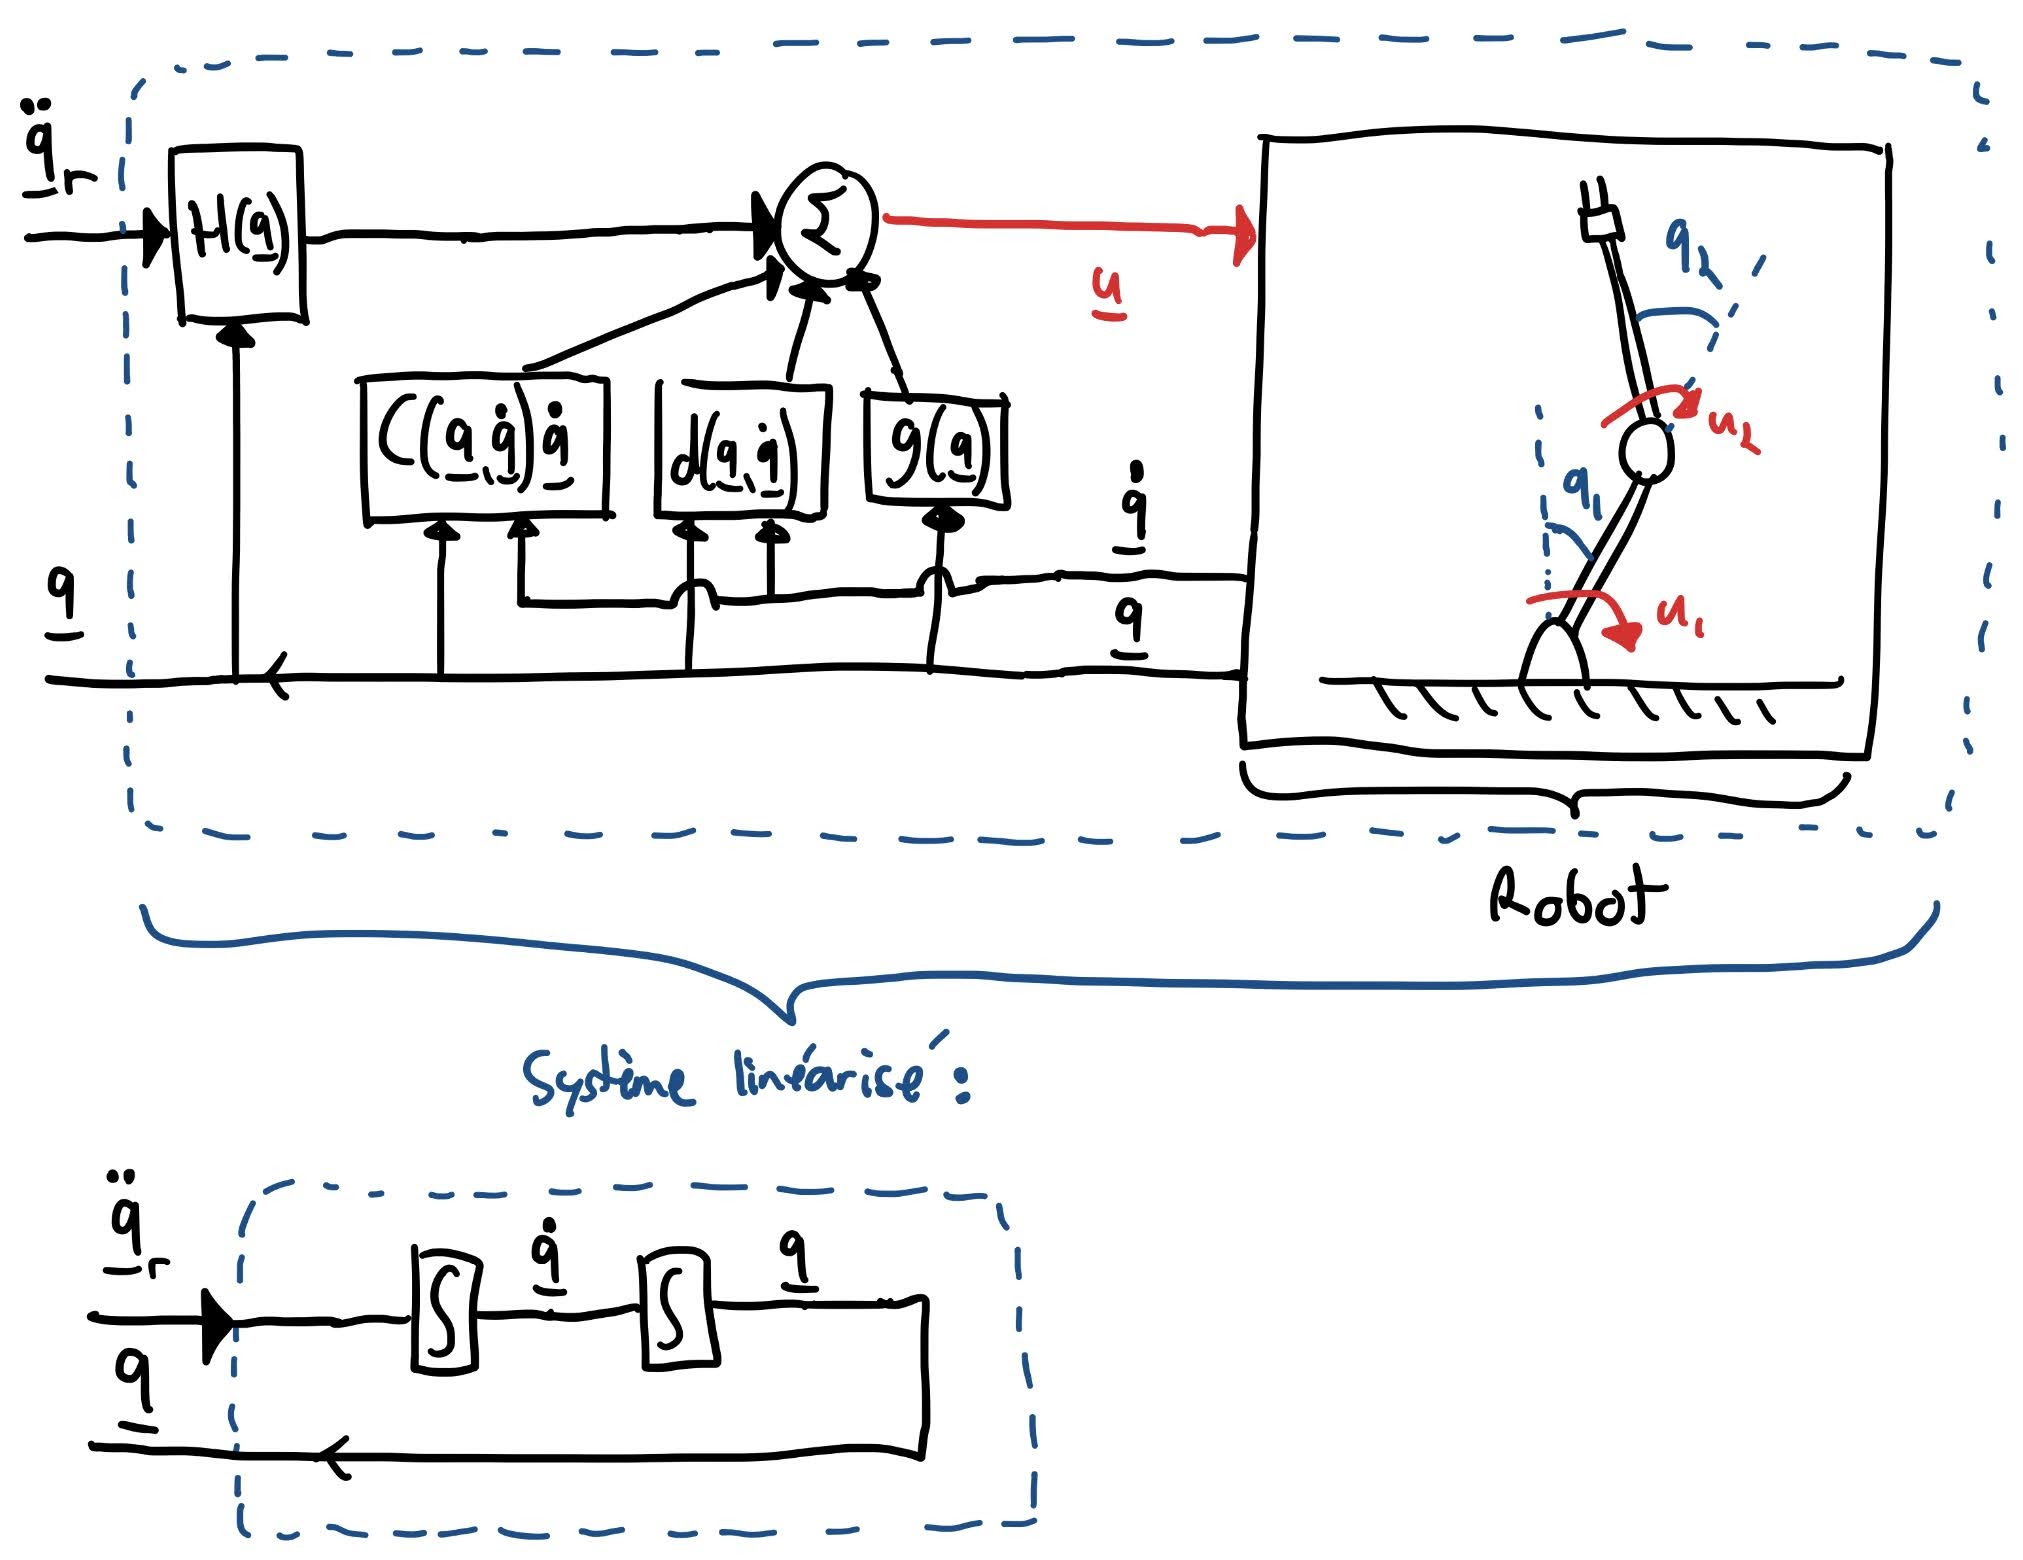
\includegraphics[width=0.75\textwidth]{fig/computedtorque.jpg}
	\caption{Couple calculé et boucle linéarisante.}
	\label{fig:computedtorque}
\end{figure}
%%%%%%%%%%%%%%%%%%%%

\subsection{Suivi de trajectoire avec le couple calculé}

Lorsqu'on désire qu'un robot suivre une certaine trajectoire, il est possible de définir la référence d'accélération $\col{\ddot{q}}_r$ comme une fonction de la trajectoire cible pour obtenir que le robot va converger sur la trajectoire. Si une trajectoire cible est définie comme une fonction du temps pour les coordonnées $\col{q}$ et leur deux premières dérivées:
%%%%%%%%%%%%%%%%%%%%%%%
\begin{align}
\text{Trajectoire désirée: } \col{\ddot{q}}_d(t) \quad \col{\dot{q}}_d(t) \quad \col{q}_d(t)
\end{align}
%%%%%%%%%%%%%%%%%%%%%%%
alors si on définie la référence d'accélération par la loi de commande suivante:
%%%%%%%%%%%%%%%%%%%%%%%
\begin{align}
\col{\ddot{q}}_r = \col{\ddot{q}}_d + 2 \zeta w 
\underbrace{\left( \col{\dot{q}}_d - \col{\dot{q}}\right)}_{ \col{\dot{q}}_e}
+ w^2
\underbrace{\left( \col{q}_d - \col{q}\right)}_{ \col{q}_e}
\end{align}
%%%%%%%%%%%%%%%%%%%%%%%
puisqu'on obtient $\col{\ddot{q}} = \col{\ddot{q}}_r$ avec la méthode du couple calculé, en combinant cette définition pour $\col{\ddot{q}}_r$ on va obtenir:
%%%%%%%%%%%%%%%%%%%%%%%
\begin{align}
\underbrace{\left( \col{\ddot{q}}_d - \col{\ddot{q}} \right)}_{ \col{\ddot{q}}_e}
 + 2 \zeta w 
\underbrace{\left( \col{\dot{q}}_d - \col{\dot{q}}\right)}_{ \col{\dot{q}}_e}
+ w^2
\underbrace{\left( \col{q}_d - \col{q}\right)}_{ \col{q}_e} = 0
\label{eq:computedtorqueerrordynamic}
\end{align}
%%%%%%%%%%%%%%%%%%%%%%%
ce qui représente une équation de la dynamique pour l'erreur d'ordre 2 qui converge exponentiellement vers zéro si on choisi $w^2>0$ et $2 \zeta w > 0$, ce qui implique que la trajectoire du robot va converger sur la trajectoire désirée. 
%%%%%%%%%%%%%%%%%%%%%%%%%
\begin{figure}[ht]
	\centering
		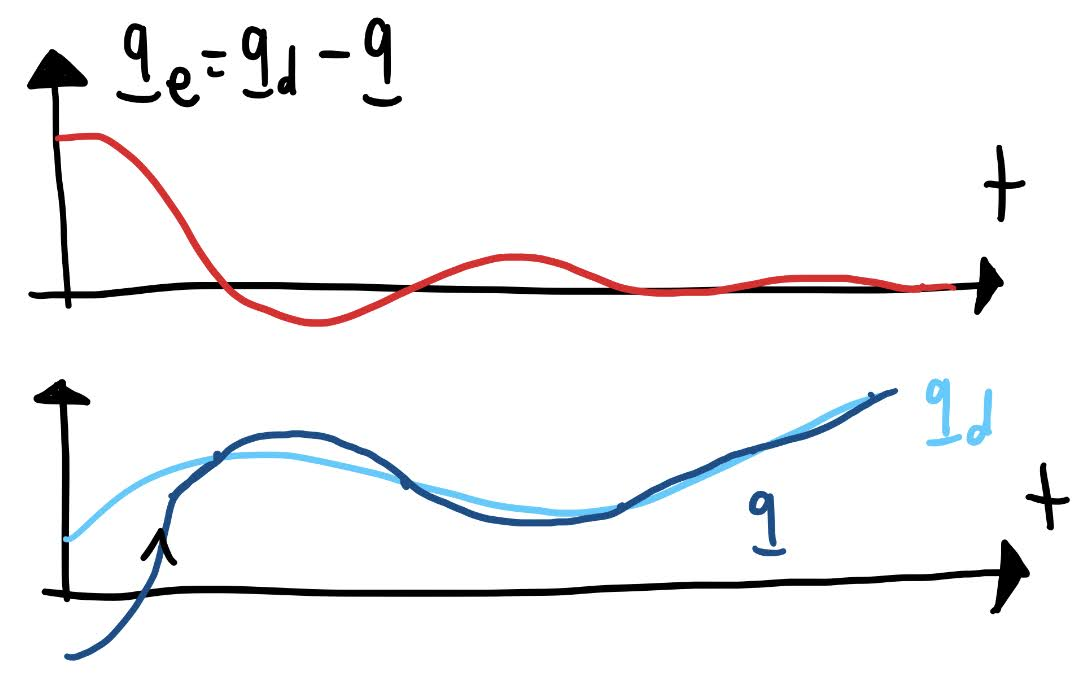
\includegraphics[width=0.50\textwidth]{fig/errordynamic.jpg}
	\caption{Dynamique de l'erreur et convergence sur la trajectoire}
	\label{fig:errordynamic}
\end{figure}
%%%%%%%%%%%%%%%%%%%%


On voit ici selon cette équation que ces paramètres dans la loi de commande ont été intégré de sorte qu'ils correspondent directement aux paramètres de fréquence naturelle et d'amortissement pour la forme standard d'une équation différentielle d'ordre deux. Ici $\zeta$ serait un paramètre de la loi de commande directement relié au dépassement et au temps d'établissement de l'erreur du système en boucle fermée et le $w$ au temps de monté et la bande passante du système en boucle fermée. De façon plus général, dans l'équation \eqref{eq:computedtorqueerrordynamic} le terme scalaire $w^2$ pourrait être remplacé par une matrice $K_p$ et le terme $2 \zeta w $ par une matrice $K_d$. Plutôt qu'avoir alors une dynamique d'erreur identique pour chaque DDL, on pourrait paramétrer des comportements plus varié. Par exemple, on pourrait choisir des matrices diagonales et les termes indépendants sur leur diagonale correspondraient à des valeurs de $w$ et $\zeta$ qui pourraient être choisi indépendemment pour chaque DDL du robot.
%%%%%%%%%%%%%%%%%%%%%%%%%
\begin{figure}[htp]
	\centering
		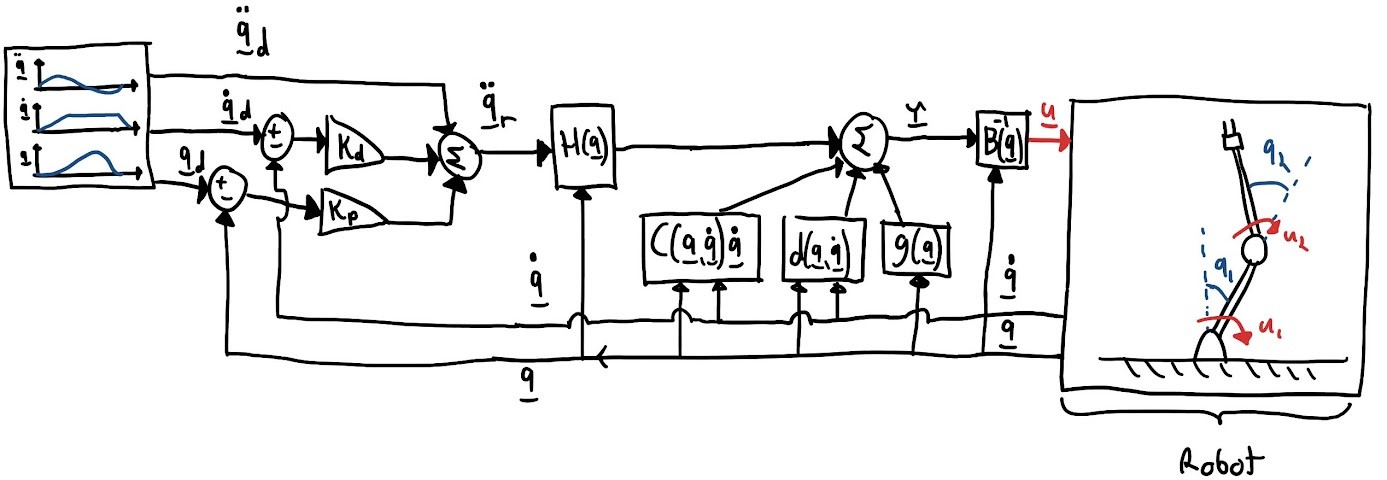
\includegraphics[width=0.99\textwidth]{fig/computedtorquetraj.jpg}
	\caption{Commande par couple calculé pour suivre une trajectoire.}
	\label{fig:computedtorquetraj}
\end{figure}
%%%%%%%%%%%%%%%%%%%%

Donc pour résumé, en assumant que notre modèle dynamique est parfait et que nous avons aussi des mesures exacte pour $\col{q}$ et $\col{\dot{q}}$, il est possible d'imposer une accélération instantanée $\col{\ddot{q}}_r$ arbitraire (si on ignore les limites des actionneurs pour le moment). Ensuite, connaissant la trajectoire cible $\col{q}_d(t)$ et ses dérivées d'ordre 1 et 2, il est possible d'imposer une accélération de sorte à avoir une erreur par rapport à la trajectoire $\col{q}_e(t)$qui tend vers zéro.







Si on regarde comment l'erreur est relié à une force demandée par la loi de commande, on peut interprété cette relation comme une matrice de rigidité, de même que pour un la relation avec la dérivé de l'erreur qui peut être interprété comme une matrice d'amortissement. Les autres termes qui ne sont pas relié à l'erreur ou l'accélération de la trajectoire cible ont tous comme rôle d'annuler des forces internes. Donc si on décortique la loi de commande, on peut regrouper les termes ansi:
%%%%%%%%%%%%%%%%%%%%%%%
\begin{align}
\col{u} &= B(\col{q})^{-1} \left[  H(\col{q}) \col{\ddot{q}}_r + C(\col{q},\col{\dot{q}}) \col{\dot{q}} + d(\col{q}, \col{\dot{q}}) + \col{g}(\col{q}) \right] \\
\col{u} &= B(\col{q})^{-1} \left[  H(\col{q}) \left( \col{\ddot{q}}_d + K_d  \col{\dot{q}}_e  + K_p \col{q}_e \right) + C(\col{q},\col{\dot{q}}) \col{\dot{q}} + d(\col{q}, \col{\dot{q}}) + \col{g}(\col{q}) \right] \\
\col{u} &= 
\underbrace{
\left[ B(\col{q})^{-1} H(\col{q})  \right] \, \col{\ddot{q}}_d 
}_{\text{Termes anticipatif}}
+ 
\underbrace{
\left[ B(\col{q})^{-1} H(\col{q}) K_d  \right] \,  \col{\dot{q}}_e 
+ 
\left[ B(\col{q})^{-1} H(\col{q}) K_p   \right] \, \col{q}_e 
}_{\text{Termes réactifs}}
+
\underbrace{
B(\col{q})^{-1} \left[ C(\col{q},\col{\dot{q}}) \col{\dot{q}} + d(\col{q}, \col{\dot{q}}) + \col{g}(\col{q}) \right]
}_{\text{Termes de compensation}}
\end{align}
%%%%%%%%%%%%%%%%%%%%%%%
et comparer à une loi de commande plus simple d'impédance dans le domaine des joints, présenté à la section \ref{sec:impcontrol}, qui est en fait aussi équivalent à utiliser des lois de commande de type proportionnelle-dérivée indépendantes pour chacun des joints. Premièrement, en plus de termes réactifs la méthode du couple calculé inclus plusieurs termes de compensation des forces internes du système, ainsi qu'un terme anticipatif si elle est utilisée pour faire du suivi de trajectoire. Ensuite, les termes réactifs ont une structure similaire, des vecteurs-colonnes d'erreur multiplient des matrices de gains. Toutefois, on remarque que dans le cas du couple calculé les matrices de gains $K_p$ et $K_d$ sont ajusté avec en étant multipliés par la matrice d'inertie $H(\col{q})$ et la matrice d'actionnement $B(\col{q})^{-1}$. Cet ajustement fait que nos gains dans les matrices $K_p$ et $K_d$ spécifient pas un lien linéaire avec un réaction en force, mais plutôt avec une réaction en accélération, pour laquelle on calcul la force nécessaire avec les matrice $H$ et $B$.


\subsection{Compensation de la friction}

Dans les méthodes de commande comme celle du couple calculé, la loi de commande vise à compenser pour tous les termes dynamiques, incluant les forces dissipatives comme la friction qui sont difficiles à modéliser. Il faut toutefois prendre garde de de pas sur-estimé l'amplitude de des forces de friction dans une boucle de compensation car cela peut rendre le système instable. Les forces dissipatives aident naturellement à la stabilité d'un système, ils dissipent de l'énergie mécanique et donc forcent le système tranquillement vers un état ou l'énergie est minimum. Une compensation de friction annule donc l'effet dissipatif de cette force, mais le problème est surtout si on surestime de niveau de friction que notre contrôleur compense trop. Dans ce cas l'effet net de la vrai friction plus la compensation par le contrôleur est une injection d'énergie dans le système, la force net pousse dans le même sense que la vitesse, ce qui risque de rendre le système instable.

%%%%%%%%%%%%%%%%%%%%%%%%%
\begin{figure}[htp]
	\centering
		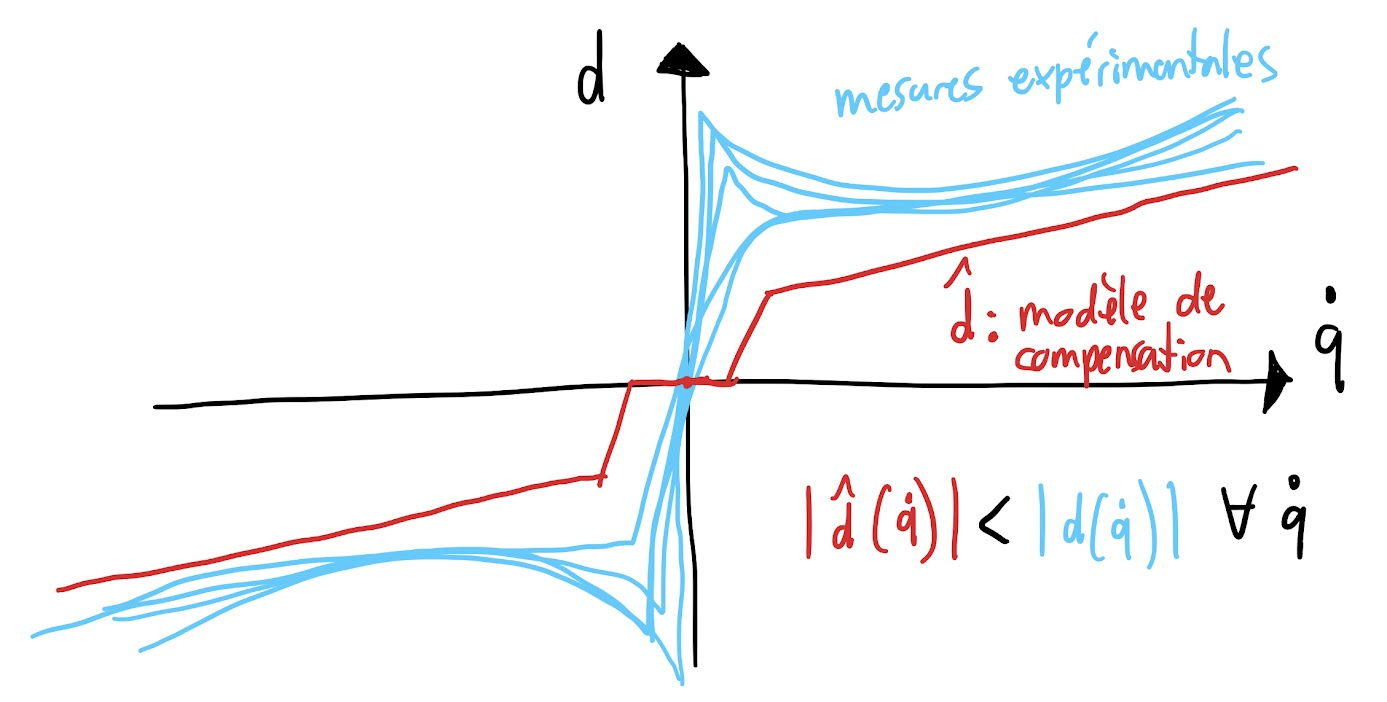
\includegraphics[width=0.75\textwidth]{fig/friction_compensation.jpg}
	\caption{Modèle de compensation de friction}
	\label{fig:friction_compensation}
\end{figure}
%%%%%%%%%%%%%%%%%%%%

Une approche pour éviter cette situation est de toujours avoir un modèle de compensation de friction qui sous-estime l'amplitude de la force de friction de façon conservateur, comme illustré à la figure \ref{fig:friction_compensation}. Mathématiquement, pour garantir que la compensation de friction ne déstabilise pas le système, on peut choisi un modèle de compensation de friction $\hat{d}$ avec une amplitude toujours inférieur à la vrai force de friction $d$ pour tout les conditions. Lorsqu'on a un modèle de friction pour chaque joint $i$ qui dépend juste de la vitesse de ce même joint, cette condition s'exprime par:
%%%%%%%%%%%%%%%%%%%%%%%%%%%%%%%%
\begin{align}
\left| \hat{d}_i(\dot{q}_i) \right| < \left| d_i(\dot{q}_i) \right| \quad \forall \dot{q}_i \quad \forall i
\end{align}
%%%%%%%%%%%%%%%%%%%%%%%%%%%%%%%%

Sous-estimer la friction dans la loi de commande du couple calculé, ou bien ne pas inclure cette compensation, ne met pas typiquement pas en péril la convergence du système sur la cible. La dynamique de l'erreur va toutefois être affecté, les propriétés d'amortissements vont être affectés. Une approche de conception peut être de retirer le terme dérivé $K_d$ de la loi de commande et le terme de compensation de friction, pour laisser la friction naturelle du système s'occuper de l'amortissement du système.  



\subsection{Suivi d'une trajectoire définie dans l'espace de la tâche}

À venir!

\subsection{Limites de la méthode}

À venir!

\subsection{Commande en impédance incluant les effets inertiels }

TODO voir notes manuscriptes alex 3 juillet 2022




\newpage
%%%%%%%%%%%%%%%%%%%%%%%%%%%%%%%%%%%%%%%%%%%%%%%
\section{Commande robuste}
%%%%%%%%%%%%%%%%%%%%%%%%%%%%%%%%%%%%%%%%%%%%%%%

La commande robuste est la science de gérer l'incertitude lors de la conception d'une loi de commande. Dans les sections précédentes, nous avions des lois de commande qui utilisaient divers propriétés du modèle cinématique et/ou dynamique du robot. Les démonstrations que ces lois de commande convergeaient assumaient alors que nos modèles utilisés dans les lois de commande étaient exacte. En pratique il y a toujours un certain degré d'incertitude, plus l'incertitude est grande plus il y a intérêt à considérer cet aspect explicitement avec des méthodes de commande robuste.

\subsection{Approche pour modéliser l'incertitude}

Dans cette section, la méthode de commande présentée est basée sur une modélisation de l'incertitude comme un vecteur de forces inconnues $\col{w}$ qui s'additionnent aux autres termes de l'équation des manipulateurs:
%%%%%%%%%%%%%%%%%%%%%%%%%%%%%%%%
\begin{align}
H(\col{q}) \col{\ddot{q}} + C(\col{q},\col{\dot{q}}) \col{\dot{q}} + d(\col{q}, \col{\dot{q}}) + \col{g}(\col{q}) = B(\col{q}) \col{u}  + \col{w}
\end{align}
%%%%%%%%%%%%%%%%%%%%%%%%%%%%%%%%
Ensuite, en fonction de bornes de valeurs minimum et maximum que peut prendre le vecteur $\col{w}$ il sera possible de synthétisé des loi de commandes qui vont garantir la convergence malgré cette incertitude.


\video{Grandes familles de méthodes de commande pour gérer l'incertitude}{https://youtu.be/hbZBF-OEZEw}

%%%%%%%%%%%%%%%%%%%%%%%%%
\begin{figure}[htp]
\vspace{-10pt}
	\centering
		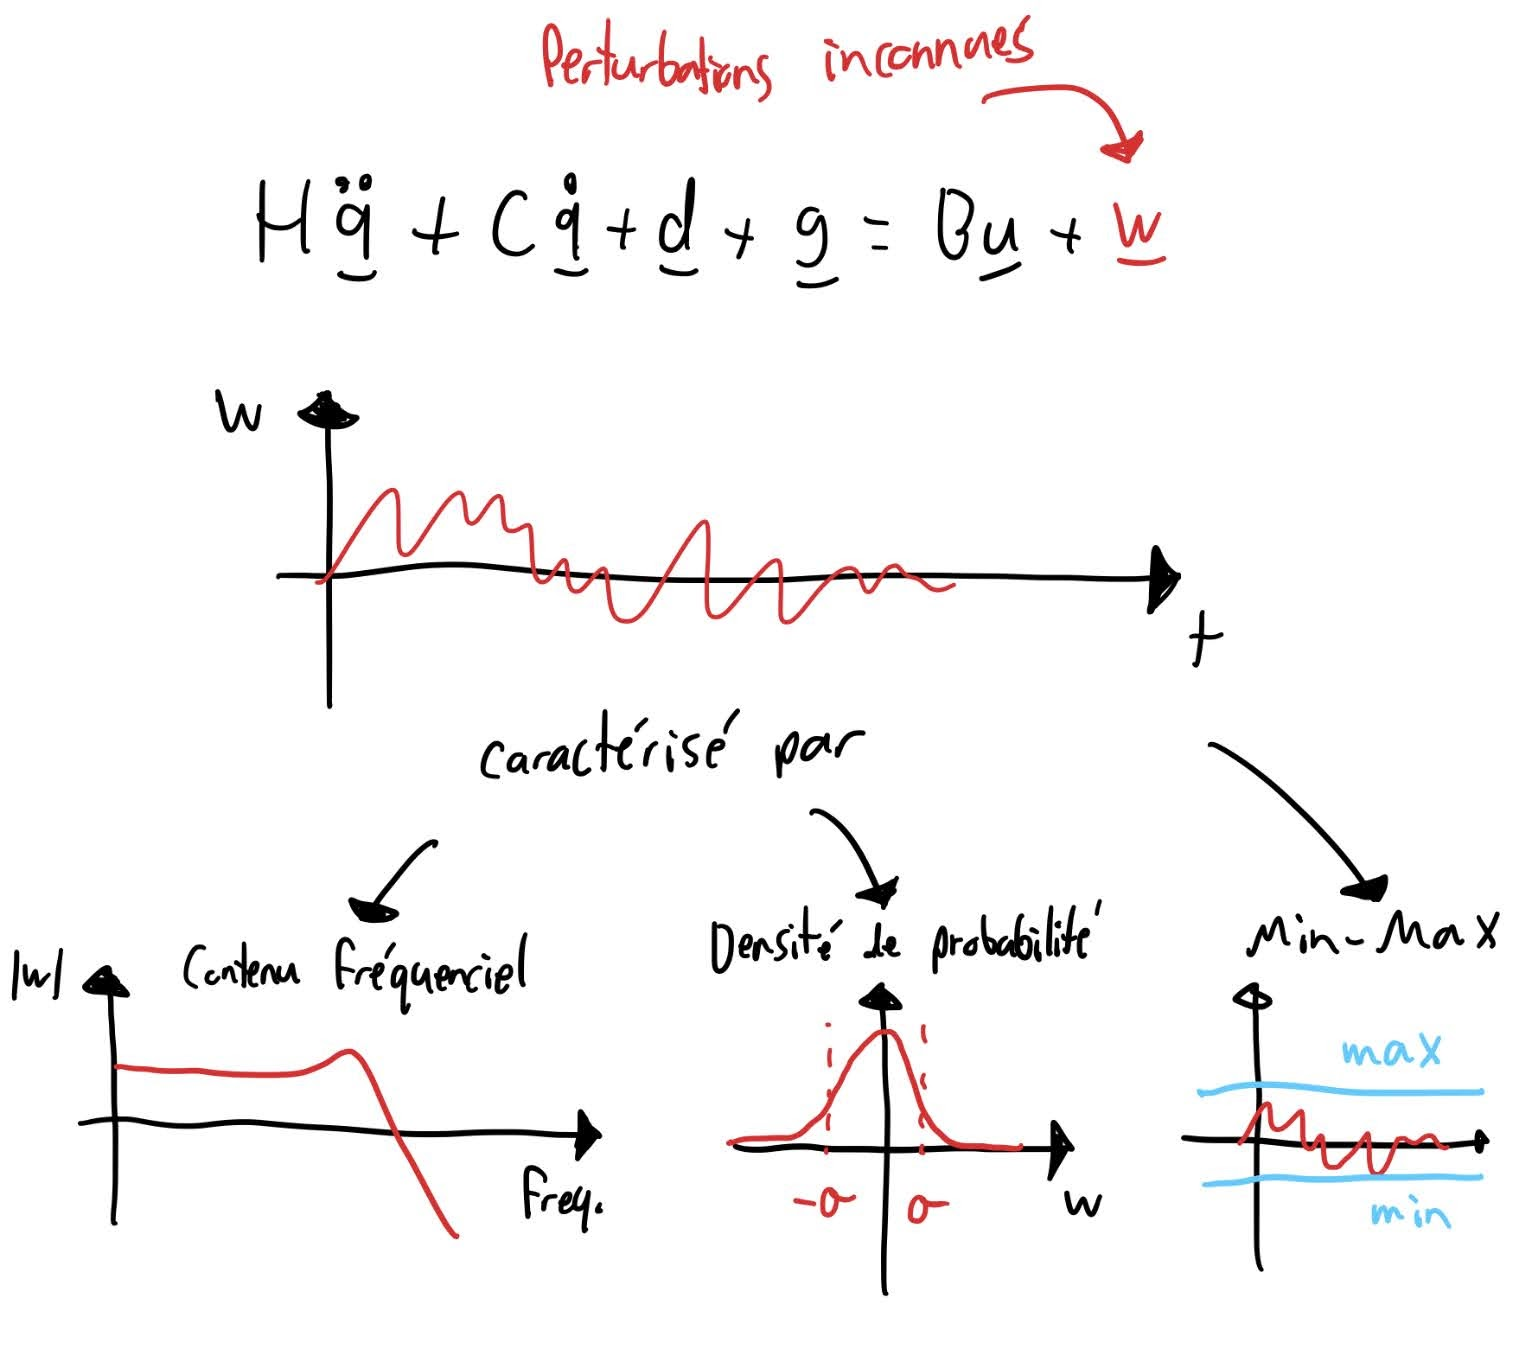
\includegraphics[width=0.7\textwidth]{fig/disturbances.jpeg}
  \vspace{-10pt}
	\caption{Divers métriques pour caractériser l'incertitude}
	\label{fig:disturbances}
\end{figure}
%%%%%%%%%%%%%%%%%%%%



\newpage
%%%%%%%%%%%%%%%%%%%%%%%%%%%%%%%%%%%%%%%%%%%%%%%
\section{Méthode du mode glissant}
%%%%%%%%%%%%%%%%%%%%%%%%%%%%%%%%%%%%%%%%%%%%%%%

La méthode du mode glissant est une approche de commande qui a comme principal attrait de pouvoir garantir la performance d'un système, malgré la présence de perturbations. En effet, si on connaît les valeurs maximums et mimimums qu'une perturbation peut prendre nous aurons une méthode pour sélectrionner des gains qui peuvent garantir la convergence.

\video{Commande avec le mode glissant}{https://youtu.be/0Asg81SBjmk}

Premièrement, la stratégie pour garantir la convergence malgré l'incertitude est basé sur le principe de "pousser" très fort sur système vers une trajectoire cible de sorte que peut importe la valeur prise par la perturbation $w$ le système est tout de même forcé sur la trajectoire. Comme illustré à la figure \ref{fig:slidingmode3}, toutes les évolutions possible du système sont toujours dans la bonne direction malgré l'incertitude avec cette approche.
%%%%%%%%%%%%%%%%%%%%%%%%%
\begin{figure}[htp]
	\centering
		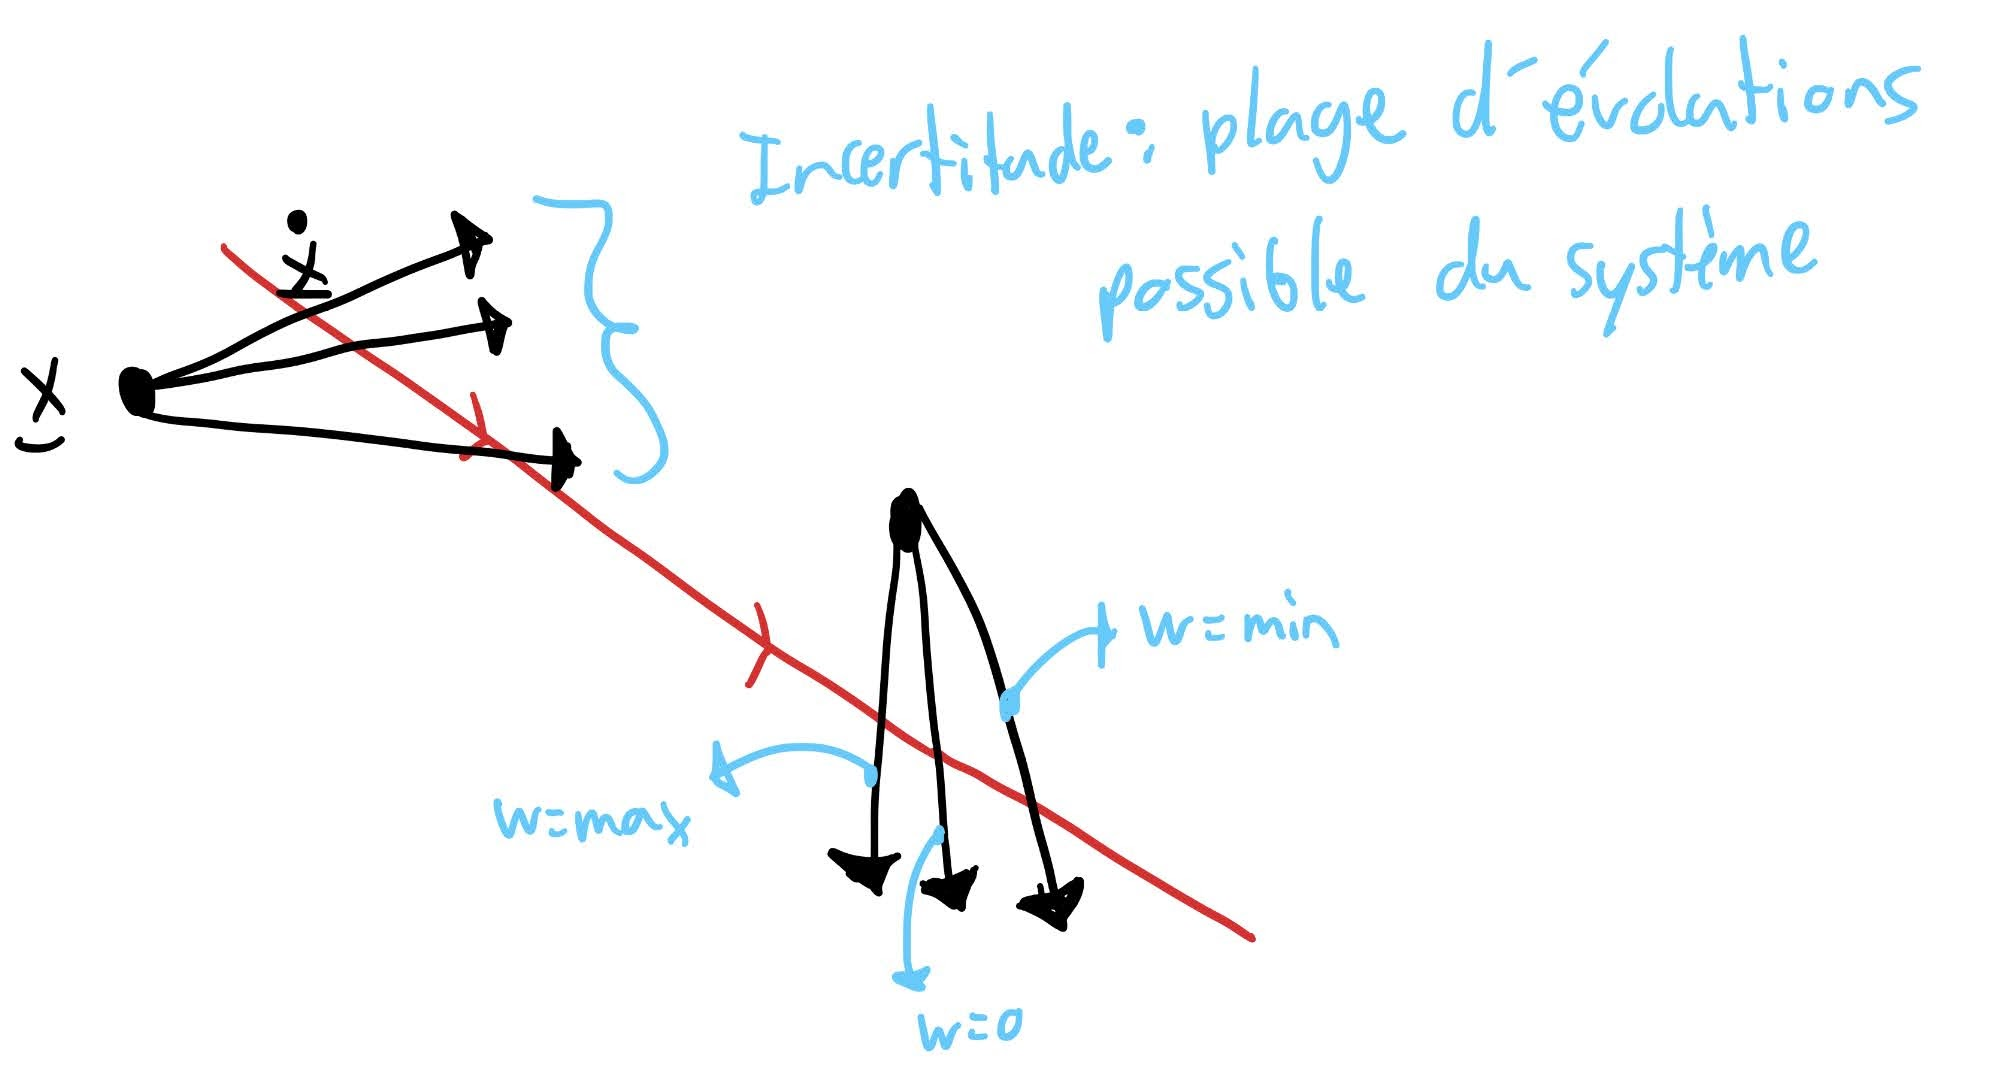
\includegraphics[width=0.70\textwidth]{fig/slidingmode3.jpeg}
	\caption{Principe de fonctionnement pour la commande par surface glissante}
	\label{fig:slidingmode3}
\end{figure}
%%%%%%%%%%%%%%%%%%%%

\colab{Robot avec une loi de commande du mode glissant}{https://colab.research.google.com/drive/1DQhoq-NbWHHI6RSf-KQXwoW7SLwfldgk?usp=sharing}

Avec la méthode de la surface glissante, le système va être forcé sur une trajectoire définie par l'équation suivante:
%%%%%%%%%%%%%%%%%%%%%%%%%%%%%%%%
\begin{align}
\col{s} = \col{\dot{q}}_e + \lambda \col{q}_e = \col{0}
\end{align}
%%%%%%%%%%%%%%%%%%%%%%%%%%%%%%%%
où les variables $s$ sont des coordonnées pour chaque DDL du système, une combinaison de la position et de la vitesse (relatif à une trajectoire cible), choisi avec un paramètre $\lambda$ de sorte que $s=0$ correspond à une trajectoire qui converge exponentiellement vers $q_e=0$. En effet, 
%%%%%%%%%%%%%%%%%%%%%%%%%%%%%%%%
\begin{align}
\col{\dot{q}}_e = - \lambda \col{q}_e \quad \text{si} \quad \col{s} = \col{0}
\end{align}
%%%%%%%%%%%%%%%%%%%%%%%%%%%%%%%%
une équation différentielle linéaire d'ordre un pour chaque DDL avec comme solution:
%%%%%%%%%%%%%%%%%%%%%%%%%%%%%%%%
\begin{align}
\col{q}_e(t) = \col{q}_e(0) \, e^{-\lambda t}
\end{align}
%%%%%%%%%%%%%%%%%%%%%%%%%%%%%%%%
Comme illustré à la figure \ref{fig:slidingmode}, les variables $s$ sont donc des coordonnées pour lesquelles le sous-ensemble $s=0$ implique une convergence exponentielle vers l'origine, c'est ce sous-ensemble qu'on appelle la surface glissante.
%%%%%%%%%%%%%%%%%%%%%%%%%
\begin{figure}[htp]
	\centering
		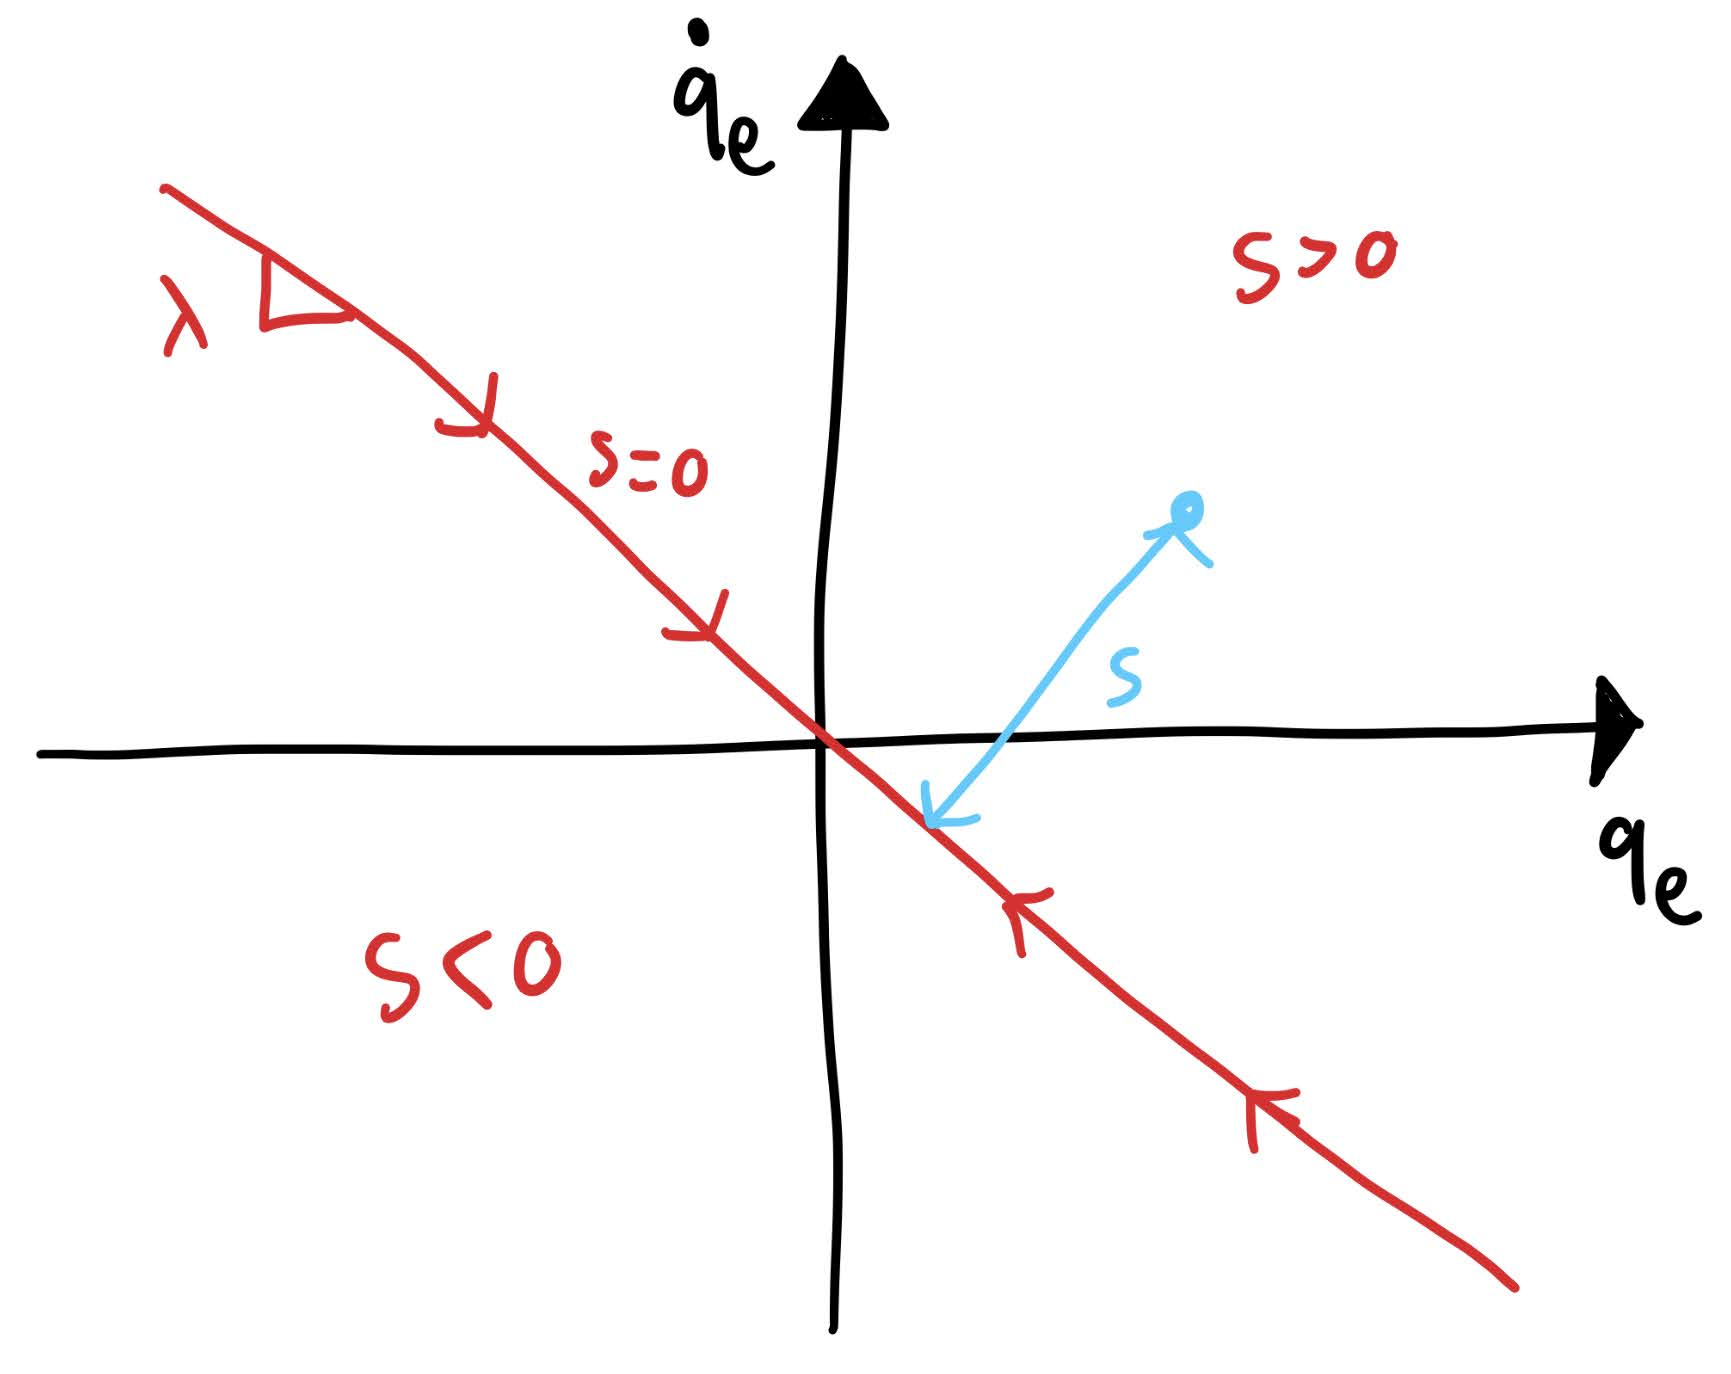
\includegraphics[width=0.50\textwidth]{fig/slidingmode.jpeg}
	\caption{Surface glissante}
	\label{fig:slidingmode}
\end{figure}
%%%%%%%%%%%%%%%%%%%%

La loi de commande par surface glissante va avoir deux composantes:
%%%%%%%%%%%%%%%%%%%%%%%%%%%%%%%%
\begin{align}
\col{u} = 
B(\col{q})^{-1} \left[
\underbrace{
\hat{\col{\tau}} 
}_{\text{ Couple équivalent }}
+ 
\underbrace{
k \sgn{ \col{s} }
}_{\text{ Couple discontinu }}
\right]
\end{align}
%%%%%%%%%%%%%%%%%%%%%%%%%%%%%%%%
Le premier terme, le couple équivalent, est un vecteur de couple calculé de façon continue qui compense plusieurs forces internes de façon similaire à la méthode du couple calculé. Le deuxième terme, est un vecteur de couple discontinus, ou chaque composant peux prendre deux valeur selon la valeur de la variable $s$ associé à ce DDL. La figure \ref{fig:slidingmode_bloc} illustre le schéma bloc de cette loi de commande.
%%%%%%%%%%%%%%%%%%%%%%%%%
\begin{figure}[htp]
	\centering
		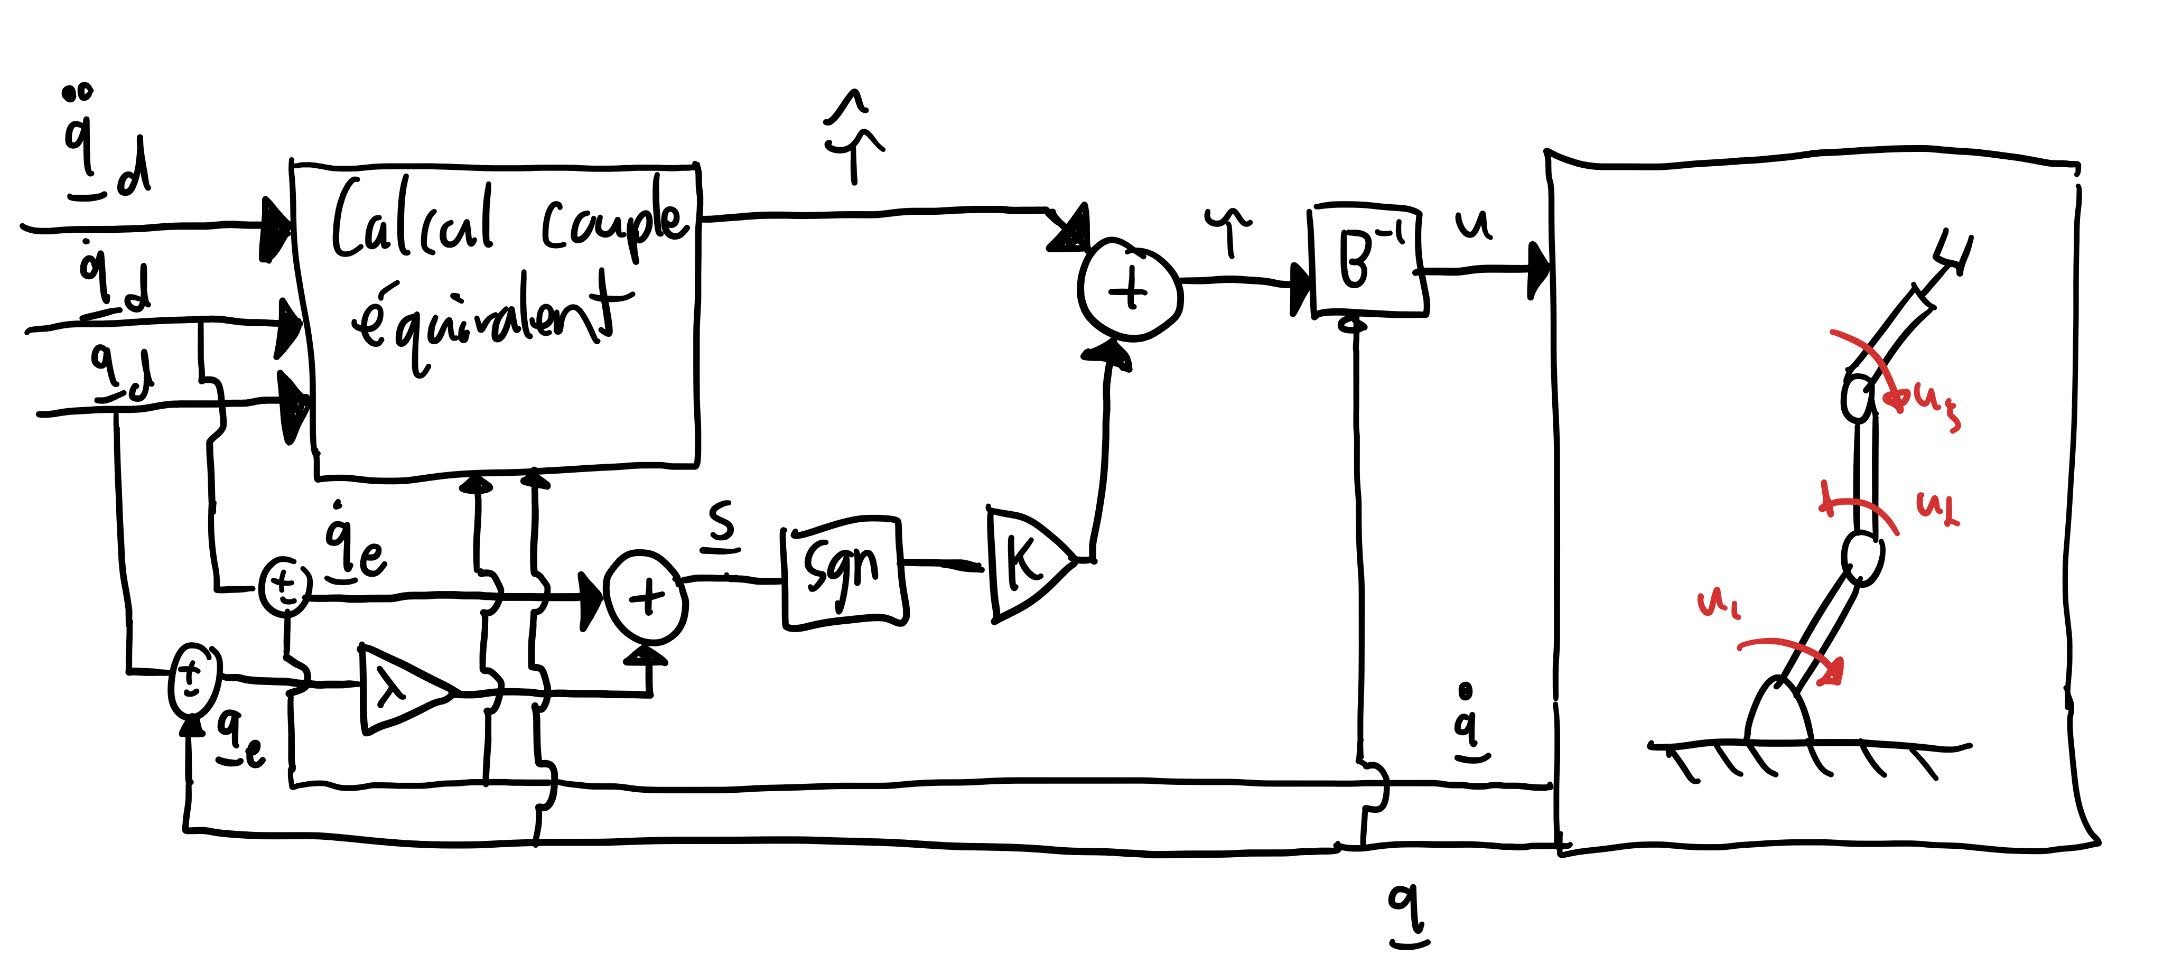
\includegraphics[width=0.90\textwidth]{fig/slidingmode_bloc.jpeg}
	\caption{Surface glissante}
	\label{fig:slidingmode_bloc}
\end{figure}
%%%%%%%%%%%%%%%%%%%%
Le couple équivalent $\hat{\col{\tau}}$ est calculé en fonction de la trajectoire désirée et l'état actuel du robot ainsi:
%%%%%%%%%%%%%%%%%%%%%%%%%%%%%%%%
\begin{align}
\hat{\col{\tau}} = H \col{\ddot{q}}_r + C \col{\dot{q}}_r + \col{d} +  \col{g}
\end{align}
%%%%%%%%%%%%%%%%%%%%%%%%%%%%%%%%
avec:
%%%%%%%%%%%%%%%%%%%%%%%%%%%%%%%%
\begin{align}
\col{\dot{q}}_r &= \col{\dot{q}}_d + \lambda \col{q}_e \\
 \col{\ddot{q}}_r &= \col{\ddot{q}}_d + \lambda \dot{q}_e \\
\end{align}
%%%%%%%%%%%%%%%%%%%%%%%%%%%%%%%%

Le signal total de commande $u$ calculé aura donc typiquement une allure continue lorsque le système est loin de la surface glissante $s=0$ et le signal fera des saut rapide entre deux valeures de $u$ lorsque le système est proche de la surface glissante, comme illustré aux figures \ref{fig:slidingmode_u} et \ref{fig:slidingmode2}. La fréquence des oscillations entre les valeurs de $u$ va dépendre en pratique de la fréquence de la boucle de contrôle. Les oscillations vont aussi se refléter sur la trajectoire du système comme un va et vient d'un côté à l'autre de la surface glissante.  
%%%%%%%%%%%%%%%%%%%%%%%%% 
\begin{figure}[htp]
	\centering
		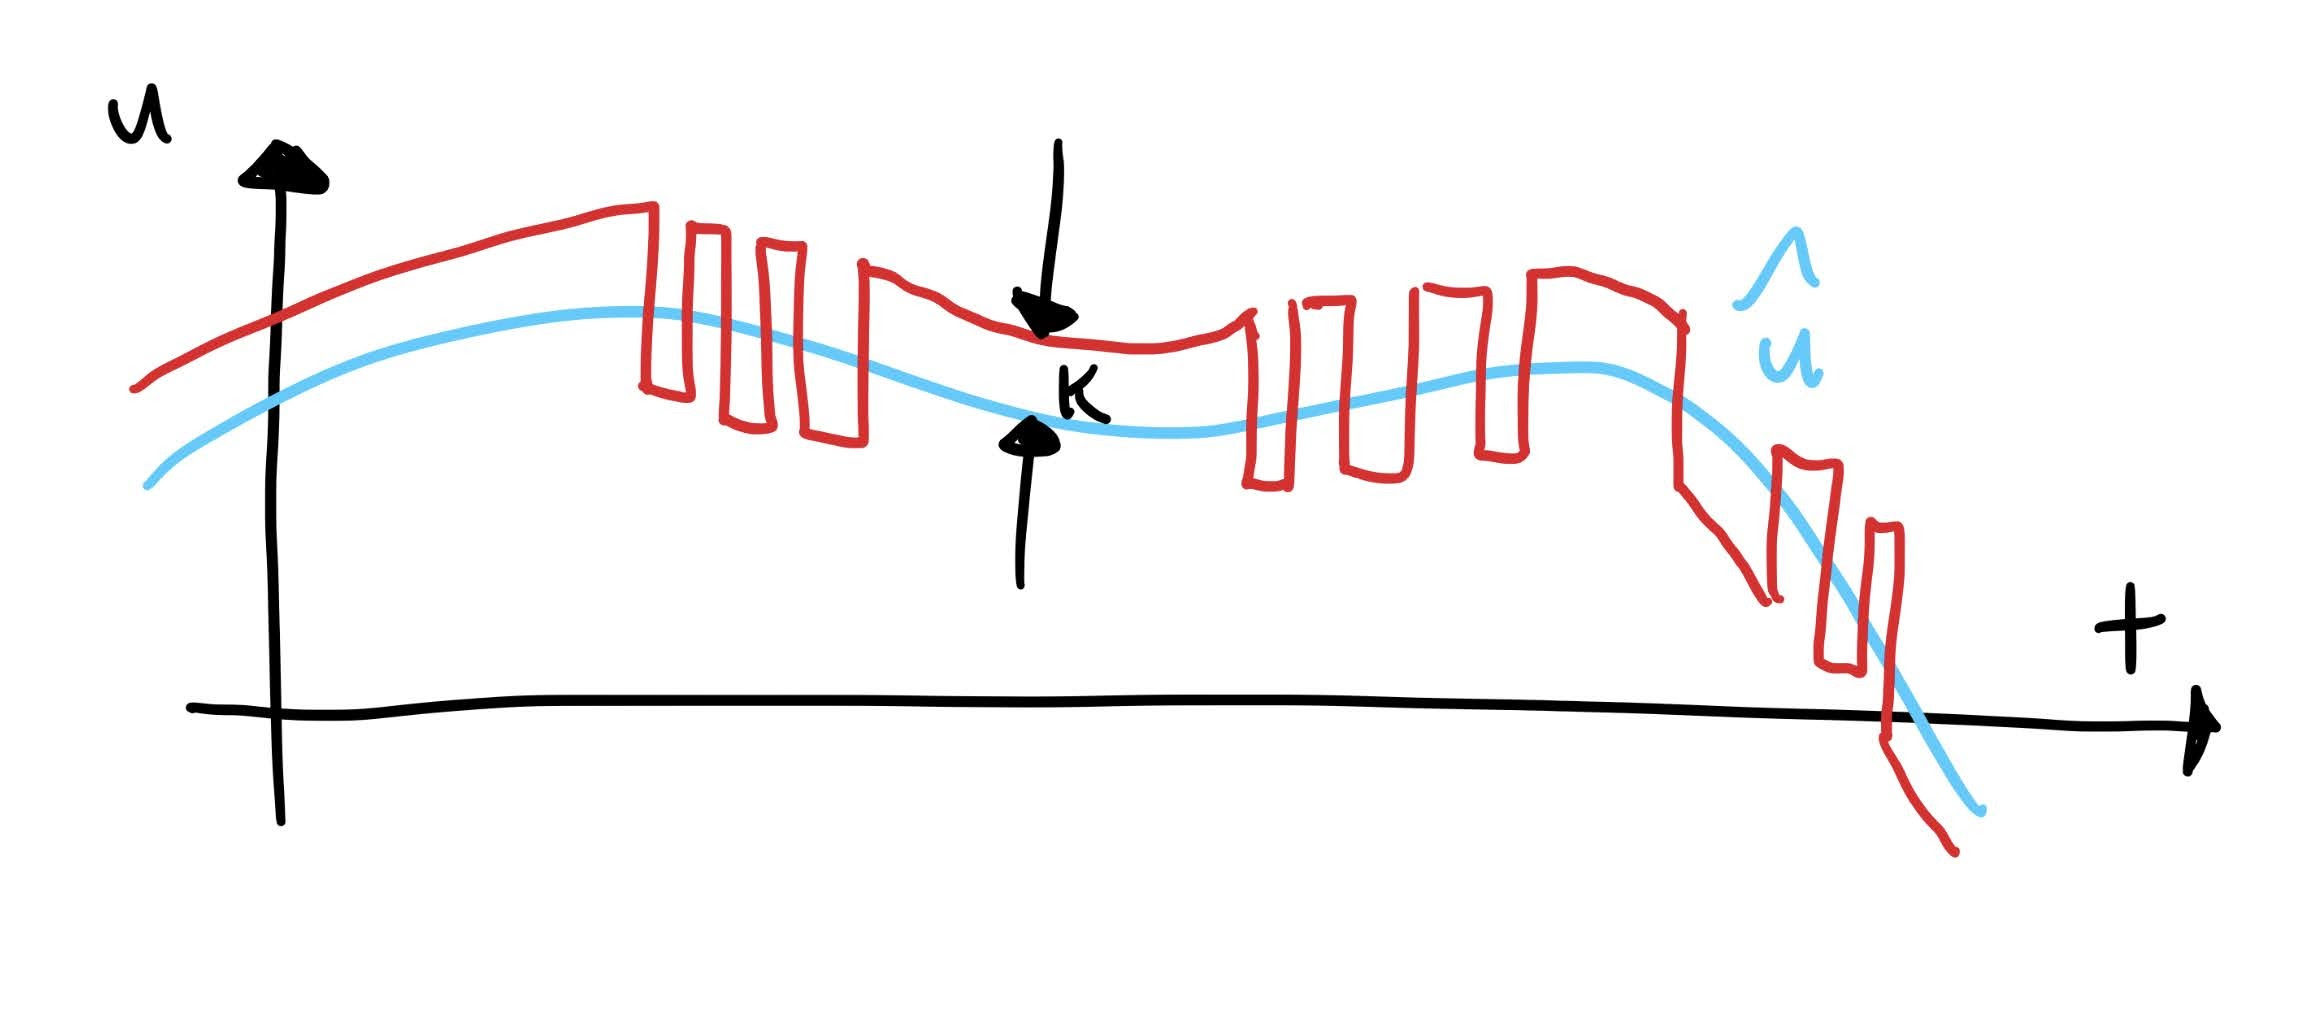
\includegraphics[width=0.80\textwidth]{fig/slidingmode_u.jpeg}
	\caption{Surface glissante}
	\label{fig:slidingmode_u}
\end{figure}
%%%%%%%%%%%%%%%%%%%%

%%%%%%%%%%%%%%%%%%%%%%%%%
\begin{figure}[htp]
	\centering
		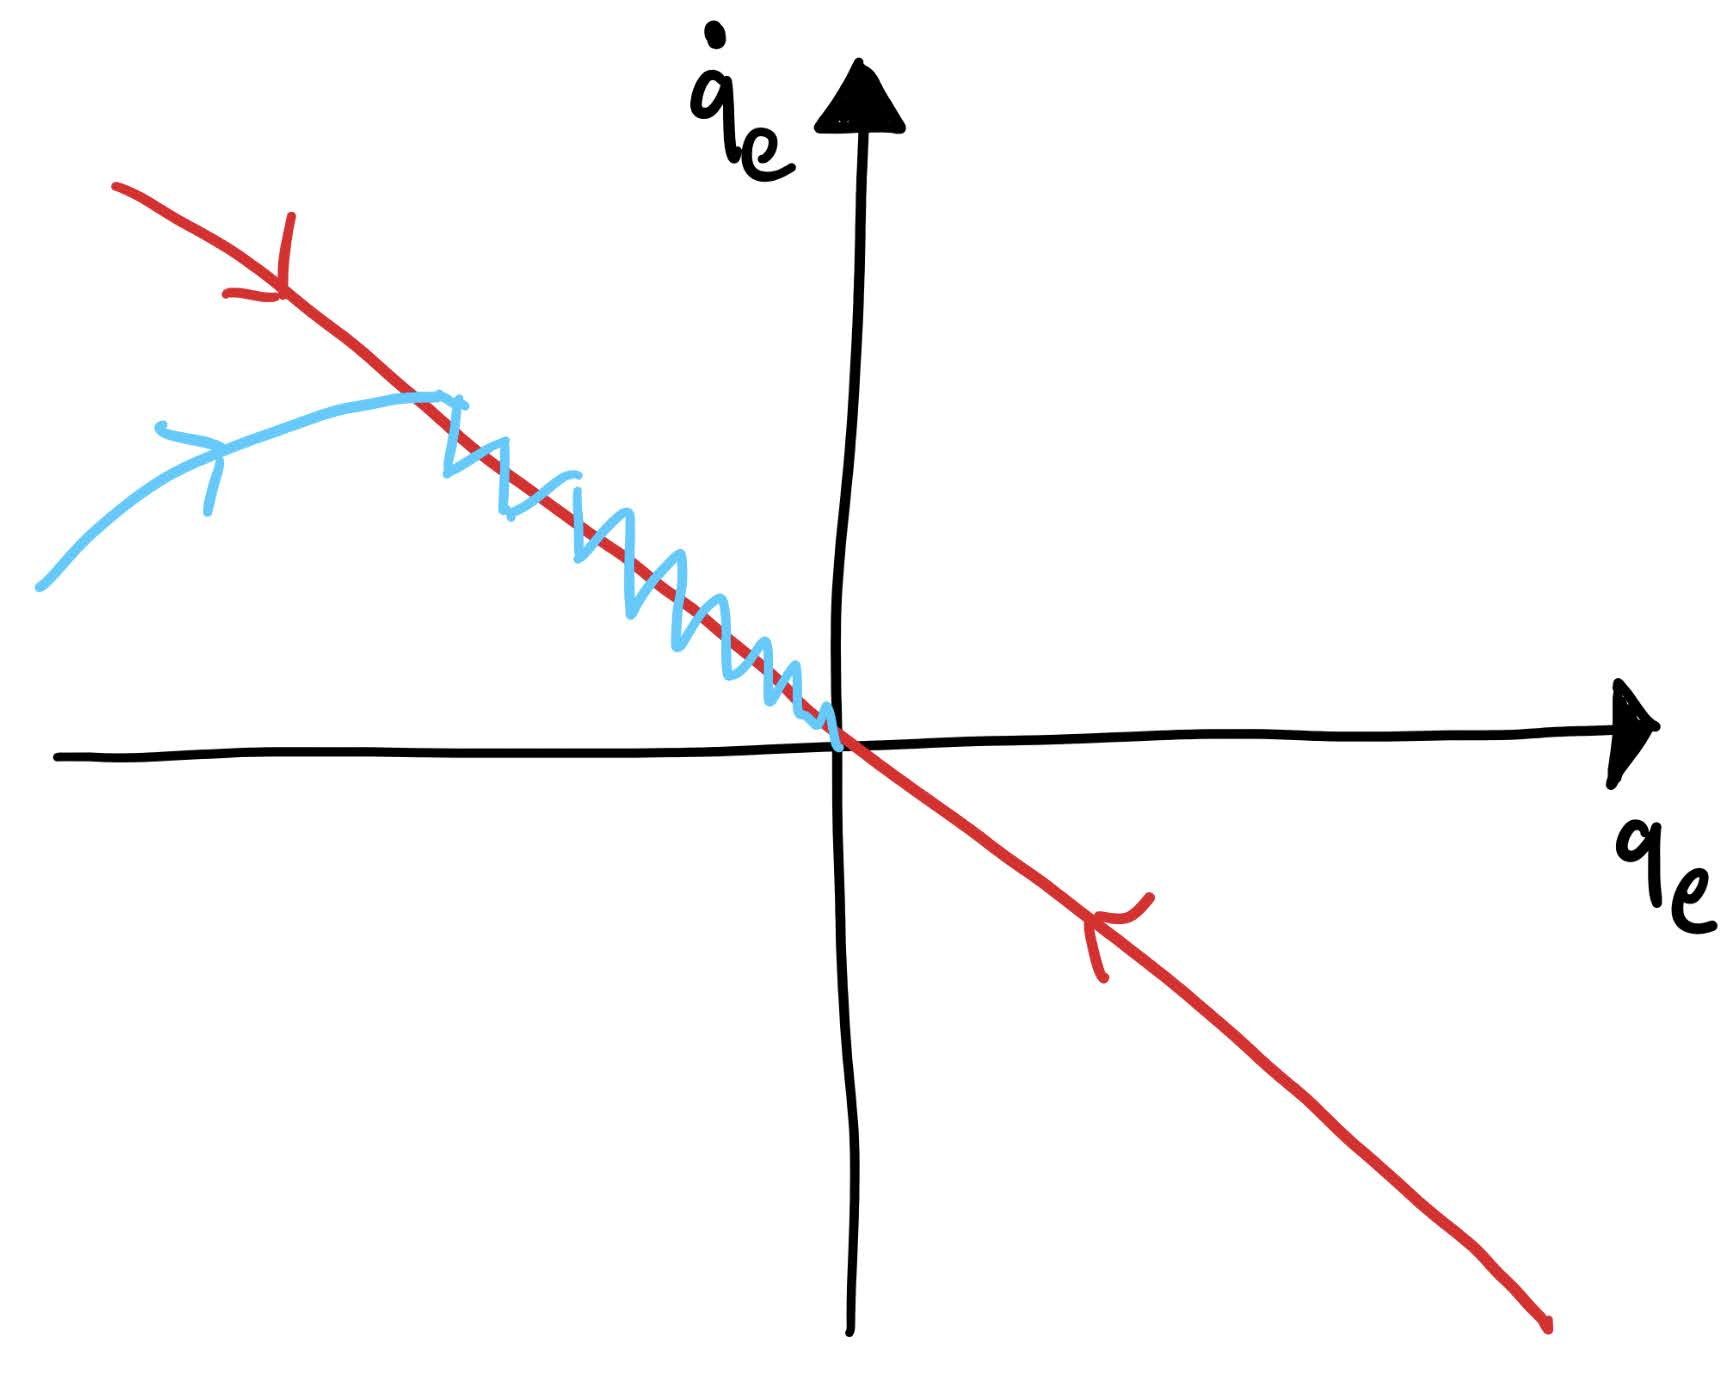
\includegraphics[width=0.50\textwidth]{fig/slidingmode2.jpeg}
	\caption{Surface glissante}
	\label{fig:slidingmode2}
\end{figure}
%%%%%%%%%%%%%%%%%%%%



\newpage
%%%%%%%%%%%%%%%%%%%%%%%%%%%%%%%%%%%%%%%%%%%%%%%
\section{Commande adaptative}
%%%%%%%%%%%%%%%%%%%%%%%%%%%%%%%%%%%%%%%%%%%%%%%

La commande dite adaptative, est une méthode de alternative pour gérer l'incertitude lorsque celle-ci est caractérisé par une erreur sur les paramètres dans l'équation dynamique. Cette approche s'applique bien pour les scénarios ou la principale source d'incertitude n'est pas des perturbations externes, mais plutôt une erreur d'estimation sur les paramètres cinématiques ou inertiels d'un système robotique. La stratégie d'une loi de commande adaptative peut se résumer en deux processus parallèles: \textbf{1) identification système:} on utilise les signaux d'entrée et de sortie du système pour effectuer une estimation en continue des paramètres du modèle, et \textbf{2) loi de commande: }on utilise l'approximation des paramètres dans une loi de commande de type couple calculé, ou autre approche basé sur un modèle du système. Cette approche est particulièrement adapté lorsqu'un système robotisé va avoir un chargement inconnu lors d'une opération par exemple. 

\video{Exemple de loi de commande adaptative}{https://youtu.be/vmYjad6SOmU}

\subsection{Approche pour modéliser l'incertitude}

Dans cette section, la méthode de commande présentée est basée sur une modélisation de l'incertitude ou on considère que des paramètres dans le modèle dynamique sont des approximations inexactes dans notre loi de commande $\hat{a}_i$. Par exemple, la masse d'un robot ou la longueur sont toujours approximé à un certain degrée lorsqu'on code une loi de commande. On va ici noter les paramètres exactes $a_i$, les approximations $\hat{a}_i$, et l'erreur sur un paramètre sera ${a_e}_i$. Les paramètres seront regroupés des vecteur-colonnes:
%%%%%%%%%%%%%%%%%%%%%%%%%%%%%%%%
\begin{align}
\underbrace{
\col{a}_e 
}_{\text{erreur}}
= 
\underbrace{
\col{a}
}_{\text{réel}}
- 
\underbrace{
\col{\hat{a}}
}_{\text{approximation}}
\end{align}
%%%%%%%%%%%%%%%%%%%%%%%%%%%%%%%%

Un atout qui sera exploité pour les systèmes dynamiques qui peuvent être représenté par l'équation des manipulateurs, est qu'on peut struturer l'équation de la dynamique comme une multiplication d'une matrice de termes connus $Y$, et du vecteur-colonnes qui regroupe tout les paramètres constants de l'équations.
%%%%%%%%%%%%%%%%%%%%%%%%%%%%%%%%
\begin{align}
H(\col{q}) \col{\ddot{q}} + C(\col{q},\col{\dot{q}}) \col{\dot{q}} + d(\col{q}, \col{\dot{q}}) + \col{g}(\col{q}) &= \col{\tau} \\
Y(\col{q},\col{\dot{q}}, \col{\ddot{q}} ) \,  \col{a} &= \col{\tau}
%Y^T(\col{q},\col{\dot{q}}, \col{\ddot{q}} ) \,  \col{\hat{a}} \approx \col{\tau}
\end{align}
%%%%%%%%%%%%%%%%%%%%%%%%%%%%%%%%
Les termes connus dans la matrice $Y$ vont être des fonctions des accélérations, vitesses et positions du robot à un instant donné. Par exemple, on pourrait avoir des termes tel que:
%%%%%%%%%%%%%%%%%%%%%%%%%%%%%%%%
\begin{align}
Y_{ii} \in \{ \ddot{q}_i \; , \; \dot{q}_i \; , \; \dot{q}_i^2 \; , \; \dot{q}_i \dot{q}_j  \; , \; \cos q_i \; , \; \sin q_i \dot{q}_i^2 , ... \}
\end{align}
%%%%%%%%%%%%%%%%%%%%%%%%%%%%%%%%
et dans le vecteur $a$ des combinaisons de paramètres géométriques, inertiel et autres qui multiplient les termes de $Y$ pour obtenir l'équation des manipulateurs:
%%%%%%%%%%%%%%%%%%%%%%%%%%%%%%%%
\begin{align}
a_i \in \{ ml^2\; , \; mgl \; , \; b_i \; , \; ... \}
\end{align}
%%%%%%%%%%%%%%%%%%%%%%%%%%%%%%%%


\newpage
%%%%%%%%%%%%%%%%%%%%%%%%%%%%%%%%%%%%%%%%%%%%%%%%%%%%%%%%%%%%%%%%
\begin{example}[Séparation des paramètres inconnus pour un pendule simple]

Pour un pendule simple avec de la friction sèche, malgré les non-linéarités dans les équations il est possible de séparer les termes connus (mesurables) qui sont mesurable et les paramètres constants:
%%%%%%%%%%%%%%%%%%%%%%%%%%%%%%%%
\begin{align}
ml^2 \ddot{q} + \mu \sgn{\dot{q}} +  mgl \sin q &= \tau \\
\underbrace{
\left[
\begin{array}{ccc}
   \ddot{q}  &  \sgn{\dot{q}} & \sin q
\end{array} \right]
}_{Y}
\,
\underbrace{
\left[
\begin{array}{c}
 ml^2 \\ \mu \\ mgl
\end{array}\right]
}_{\col{a}}
&= \tau
\end{align}

Si on mesure l'angle $q$ (et ses dérivés) on peut construire tout les termes de la matrice $Y$. Les paramètres constants sont impliqué linéairement par rapport aux termes de $Y$.
%%%%%%%%%%%%%%%%%%%%%%%%%%%%%%%%
\end{example}
%%%%%%%%%%%%%%%%%%%%%%%%%%%%%%%%


\subsection{Loi de commande}
Cette section présente une approche de commande adaptative générique pour un système pleinement actionné représenté par l'équation des manipulateurs. La loi de commande a une structure similaire aux lois de commandes présenté dans ce chapitre: un terme de compensation de dynamique et un terme supplémentaire pour garantir la convergence sur une cible. Ici la grande différence est que le terme de compensation dynamique est calculé avec l'approximation actuel des paramètres inconnus $\col{\hat{a}}$:
%%%%%%%%%%%%%%%%%%%%%%%%%%%%%%%%
\begin{align}
\col{\tau} = 
\underbrace{
Y_r \hat{\col{a}}
}_{\text{compensation dynamique}}
+
\underbrace{
K \col{s}
}_{\text{rétroaction de type PD}}
\end{align}
%%%%%%%%%%%%%%%%%%%%%%%%%%%%%%%%
où $K$ est une matrice de paramètres de gains. 

Ensuite, l'approximation des paramètres inconnus va être continuellement mise à jour avec l'équation suivante qui dicte la dérivée temporelle de nos approximations comme une fonction de variables mesurables:
%%%%%%%%%%%%%%%%%%%%%%%%%%%%%%%%
\begin{align}
\dot{\hat{\col{a}}} = - P^T Y_r^T \col{s}
\end{align}
%%%%%%%%%%%%%%%%%%%%%%%%%%%%%%%%
où $P$ est une matrice inversible de gains d'adaptation. 
La loi de commande va ici avoir des états internes et une mémoire (la consigne $\col{\tau}$ peut prendre différentes valeur pour un état donné du système physique selon l'historique). Le vecteur d'approximation des paramètres inconnus $\col{\hat{a}}$ constitue des états internes qui vont être incrémenté continuellement avec un schéma d'intégration:
%%%%%%%%%%%%%%%%%%%%%%%%%%%%%%%%
\begin{align}
\hat{\col{a}}(t) = \int_{t_0}^{t} \left( - P^T Y_r^T \col{s} \right) dt   + \hat{\col{a}}(t_0)
\end{align}
%%%%%%%%%%%%%%%%%%%%%%%%%%%%%%%%
Des variables intermédiaires on été utilisés dans les équations précédantes et sont définies si dessous:
%%%%%%%%%%%%%%%%%%%%%%%%%%%%%%%%
\begin{align}
\col{q}_e        &= \col{q}_d - \col{q} \\
\dot{\col{q}}_r  &= \dot{\col{q}}_d + \lambda \col{q}_e  \\
\ddot{\col{q}}_r &= \ddot{\col{q}}_d + \lambda \dot{\col{q}}_e \\
\col{s}          &= \dot{\col{q}}_e + \lambda \col{q}_e = \dot{\col{q}}_r - \dot{\col{q}}
\end{align}
%%%%%%%%%%%%%%%%%%%%%%%%%%%%%%%%
Il est aussi à noter qu'il y a deux version de la matrice $Y$:
%%%%%%%%%%%%%%%%%%%%%%%%%%%%%%%%
\begin{align}
Y \col{a}   &=  H \col{\ddot{q}} + C \col{\dot{q}} + \col{d} + \col{g}  = \col{\tau} \\
Y_r \col{a} &= H \col{\ddot{q}}_r + C \col{\dot{q}}_r + \col{d} + \col{g}  
\end{align}
%%%%%%%%%%%%%%%%%%%%%%%%%%%%%%%%
$Y$ dépend seulement des positions, vitesses et accélération, alors que $Y_r$ n'utilise pas l'accélération réelle mais est plutôt basé sur l'erreur:
%%%%%%%%%%%%%%%%%%%%%%%%%%%%%%%%
\begin{align}
Y &= Y(\ddot{\col{q}},\dot{\col{q}},\col{q}) \\
Y_r &= Y_r(\ddot{\col{q}}_r,\dot{\col{q}}_r,\dot{\col{q}},\col{q})
\end{align}
%%%%%%%%%%%%%%%%%%%%%%%%%%%%%%%%




\colab{Commande adaptative pour un pendule simple}{https://colab.research.google.com/drive/1J8C-CvJdrhDU4q1294057Qopn3tnEBNi?usp=sharing}


\begin{proof}
Il est possible de démontrer que la loi de commande proposée dans cette section, incluant la loi d'adaptation, va faire converger le système sur la trajectoire désirée pour n'importe quel valeur initial d'estimation des paramètres $\col{\hat{a}}$. 

Avec comme fonction de Lyapunov:
%%%%%%%%%%%%%%%%%%%%%%%%%%%%%%%%
\begin{align}
V = \frac{1}{2} \col{s}^T H \col{s} + \frac{1}{2} \col{\hat{a}}^T P^{-1} \col{a}_e
\end{align}
%%%%%%%%%%%%%%%%%%%%%%%%%%%%%%%%

Il est possible de démontrer que la dérivée temporelle va être strictement négative sauf lorsque $\col{s} = \col{0}$:
%%%%%%%%%%%%%%%%%%%%%%%%%%%%%%%%
\begin{align}
\dot{V} &= \col{s}^T \left( H \col{\dot{s}} + 2 \dot{H} \col{s}  \right) + \col{\dot{\hat{a}}}^T P^{-1} \col{a}_e \\
\dot{V} &= \col{s}^T \left( H \ddot{\col{q}}_r - \col{\tau} + C \dot{\col{q}} +  \col{d} + \col{g} + 2 \dot{H} \dot{\col{q}}_r - 2 \dot{H} \dot{\col{q}} \right) + \col{\dot{\hat{a}}}^T P^{-1} \col{a}_e  \\
\dot{V} &= - \col{s}^T K \col{s} + 
\underbrace{
\col{s}^T Y_r \col{a}_e + \col{\dot{\hat{a}}}^T P^{-1} \col{a}_e 
}_{0} \\
\dot{V} &= - \col{s}^T K \col{s} < 0 \quad \forall \quad \col{s} \neq \col{0}
\end{align} 
%%%%%%%%%%%%%%%%%%%%%%%%%%%%%%%%
En utilisant le lemme de Barbalat (voir livre de commande non-linéaire), il est possible de conclure que $\col{s} \rightarrow \col{0}$ ce qui implique qu'on va converger sur la trajectoire car $\col{q}_e \rightarrow \col{0}$. Il est toutefois important de noter que cela n'implique pas que $\col{a}_e \rightarrow \col{0}$.
\end{proof}


%%%%%%%%%%%%%%%%%%%%%%%%%%%%%%%%%%%%%%%%%%%%%%%%%%%%%%%%%%%%%%%%
\begin{example}[Loi de commande et d'adaptation pour un pendule simple]

Si on reprend l'exemple du pendule simple décrit par l'équation suivante:
%%%%%%%%%%%%%%%%%%%%%%%%%%%%%%%%
\begin{align}
\underbrace{
\left[
\begin{array}{ccc}
   \ddot{q}  &  \sgn{\dot{q}} & \sin q
\end{array} \right]
}_{Y}
\,
\underbrace{
\left[
\begin{array}{c}
 ml^2 \\ \mu \\ mgl
\end{array}\right]
}_{\col{a}}
&= \tau
\end{align}
%%%%%%%%%%%%%%%%%%%%%%%%%%%%%%%%

La loi de commande serait alors:
%%%%%%%%%%%%%%%%%%%%%%%%%%%%%%%%
\begin{align}
\tau &= Y_r \hat{\col{a}} + 
K s \\
\tau &=
\left[ \begin{array}{ccc}
   \ddot{q}_r  &  \sgn{\dot{q}} & \sin q
\end{array} \right] 
\left[
\begin{array}{c}
 \widehat{ml^2} \\  \widehat{\mu} \\  \widehat{mgl}
\end{array}\right]
+ K ( \dot{q}_e + \lambda q_e ) \\
\tau &=
 \widehat{ml^2} (\ddot{q}_d + \lambda \dot{q}_e) +
 \widehat{\mu} \sgn{\dot{q}} + \widehat{mgl} \sin q
+ K ( \dot{q}_e + \lambda q_e ) \\
\tau &=
 \widehat{ml^2} \ddot{q}_d  +
 \widehat{\mu} \sgn{\dot{q}} + \widehat{mgl} \sin q
+ ( \widehat{ml^2} \lambda +  K ) \dot{q}_e + K \lambda q_e 
\end{align}
%%%%%%%%%%%%%%%%%%%%%%%%%%%%%%%%
et la loi d'adaptation serait alors:
%%%%%%%%%%%%%%%%%%%%%%%%%%%%%%%%
\begin{align}
\dot{\hat{\col{a}}} &= - P^T Y_r^T s \\
\frac{d}{dt} \left[ \begin{array}{c}
 \widehat{ml^2} \\  \widehat{\mu} \\  \widehat{mgl}
\end{array} \right]
&= - \left[ \begin{array}{ccc}
p_1 &0&0 \\ 0& p_2 &0 \\ 0& 0& p_3
\end{array} \right]
\left[ \begin{array}{c}
   \ddot{q}_r  \\  \sgn{\dot{q}} \\ \sin q
\end{array} \right] ( \dot{q}_e + \lambda q_e ) \\
\frac{d}{dt} \left[ \begin{array}{c}
 \widehat{ml^2} \\  \widehat{\mu} \\  \widehat{mgl}
\end{array} \right]
&= - 
\left[ \begin{array}{c}
   p_1 (\ddot{q}_d + \lambda \dot{q}_e)  \\  p_2 \sgn{\dot{q}} \\ p_3 \sin q
\end{array} \right] ( \dot{q}_e + \lambda q_e )
\end{align}
%%%%%%%%%%%%%%%%%%%%%%%%%%%%%%%%

\end{example}
%%%%%%%%%%%%%%%%%%%%%%%%%%%%%%%%



\subsection{Estimation avec les moindres carrés}

À venir!

Pourquoi ne pas plutôt estimer les paramètres avec un schéma des moindres carrés? Est-ce qu'il y a un enjeux de stabilité?

\subsection{Apprentissage machine}

Le principe d'adaptation peut être vue comme un forme d'apprentissage machine en ligne. Avec une loi de commande adaptative, on chercher à "apprendre" automatiquement les bons paramètres $\col{a}$ à l'aide des données observées. La matrice $P$ peut être vue comme une forme de paramètres de taux d'apprentissage.

À venir!

\subsection{Adaptation à des erreurs dans la matrice jacobienne}

À venir!



\newpage
%%%%%%%%%%%%%%%%%%%%%%%%%%%%%%%%%%%%%%%%%%%%%%%
\section{Commande hybride en position et force}
%%%%%%%%%%%%%%%%%%%%%%%%%%%%%%%%%%%%%%%%%%%%%%%


\newpage
%%%%%%%%%%%%%%%%%%%%%%%%%%%%%%%%%%%%%%%%%%%%%%%
\section{Analyse de stabilité}
%%%%%%%%%%%%%%%%%%%%%%%%%%%%%%%%%%%%%%%%%%%%%%%

\video{Introduction à l'analyse de stabilité pour les systèmes non-linéaires}{https://youtu.be/q0Oqa5J3zEk}


\newpage
%%%%%%%%%%%%%%%%%%%%%%%%%%%%%%%%%%%%%%%%%%%%%%%
\section{Commande optimale}
%%%%%%%%%%%%%%%%%%%%%%%%%%%%%%%%%%%%%%%%%%%%%%%

\video{Exemple de loi de commande optimale pour un double intégrateur}{https://youtu.be/wKjEAXFvXlQ}

\video{Exemple de loi de commande optimale pour un pendule}{https://youtu.be/iUlkKdEK_dU}

\colab{Démo d'introduction aux méthodes de commande optimales}{https://colab.research.google.com/drive/1wXmlIqNGC2LrJkmyj56Y109b5ZDHVboq?usp=sharing}